\documentclass[tikz,border=5pt]{standalone}
\usepackage[T1]{fontenc}
\usepackage{lmodern,amsmath,amssymb}
\usetikzlibrary{arrows.meta,calc,positioning,fit,backgrounds,shapes.geometric,matrix,decorations.pathreplacing,patterns}
\definecolor{ink}{gray}{0.08}
\definecolor{wash}{gray}{0.965}
\definecolor{soft}{gray}{0.45}
\tikzset{box/.style={draw=ink,line width=.65pt,fill=white,align=center,inner sep=4pt,outer sep=0pt,font=\small},flow/.style={draw=ink,line width=.65pt,-{Latex[length=1.8mm,width=1.3mm]},rounded corners=2pt},annotation/.style={font=\scriptsize,text=soft,align=center},groupbox/.style={draw=soft,dashed,line width=.45pt,fill=wash}}
\begin{document}
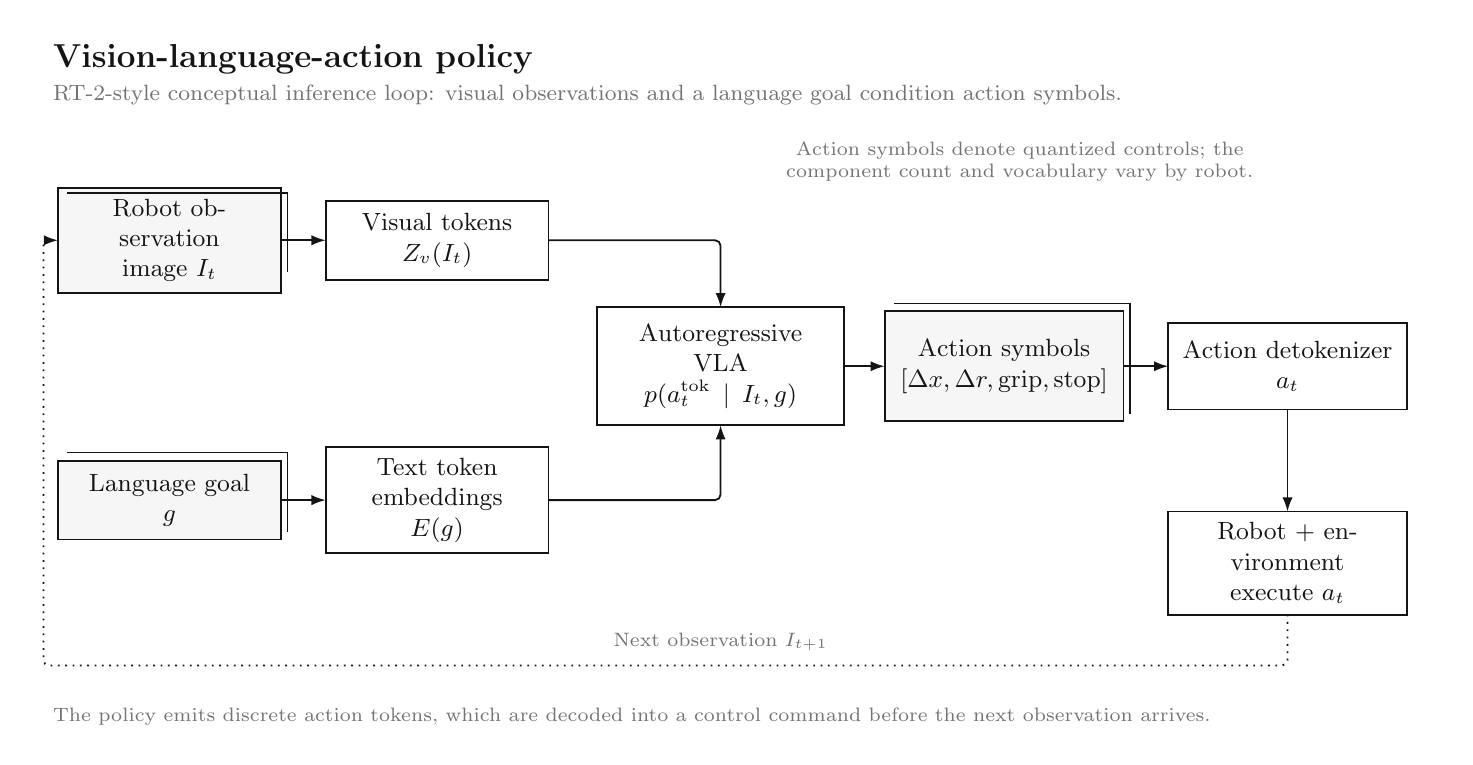
\begin{tikzpicture}[x=1cm,y=-1cm,font=\rmfamily,text=ink]

\path[use as bounding box] (0,0) rectangle (18,9);
\node[anchor=west,font=\large\bfseries] at (.2,.4) {Vision-language-action policy};
\node[anchor=west,font=\footnotesize,text=soft] at (.2,.85) {RT-2-style conceptual inference loop: visual observations and a language goal condition action symbols.};
\begin{pgfonlayer}{background}
\end{pgfonlayer}
\node[box,fill=wash,minimum width=2.8cm,minimum height=1cm,text width=2.55cm] (obs) at (1.8,2.7) {Robot observation\\image $I_t$};
\draw[ink,line width=.4pt] (0.5000000000000001,2.1) -- (3.3000000000000003,2.1) -- (3.3000000000000003,3.1);
\node[box,minimum width=2.8cm,minimum height=1.0cm,text width=2.55cm] (vision) at (5.2,2.7) {Visual tokens\\$Z_v(I_t)$};
\node[box,fill=wash,minimum width=2.8cm,minimum height=1cm,text width=2.55cm] (goal) at (1.8,6.0) {Language goal\\$g$};
\draw[ink,line width=.4pt] (0.5000000000000001,5.4) -- (3.3000000000000003,5.4) -- (3.3000000000000003,6.4);
\node[box,minimum width=2.8cm,minimum height=1.0cm,text width=2.55cm] (text) at (5.2,6.0) {Text token embeddings\\$E(g)$};
\node[box,minimum width=3.1cm,minimum height=1.5cm,text width=2.85cm] (policy) at (8.8,4.3) {Autoregressive VLA\\$p(a_t^{\mathrm{tok}}\mid I_t,g)$};
\node[box,fill=wash,minimum width=3.0cm,minimum height=1.4cm,text width=2.75cm] (actions) at (12.4,4.3) {Action symbols\\$[\Delta x,\Delta r,\mathrm{grip},\mathrm{stop}]$};
\draw[ink,line width=.4pt] (11.0,3.4999999999999996) -- (14.0,3.4999999999999996) -- (14.0,4.9);
\node[box,minimum width=3.0cm,minimum height=1.1cm,text width=2.75cm] (decode) at (16.0,4.3) {Action detokenizer\\$a_t$};
\node[box,minimum width=3.0cm,minimum height=1.1cm,text width=2.75cm] (robot) at (16.0,6.8) {Robot + environment\\execute $a_t$};
\begin{pgfonlayer}{background}
\draw[flow] (obs.east) -- (vision.west);
\draw[flow] (goal.east) -- (text.west);
\draw[flow] (vision.east) -- (8.8,2.7) -- (policy.north);
\draw[flow] (text.east) -- (8.8,6.0) -- (policy.south);
\draw[flow] (policy.east) -- (actions.west);
\draw[flow] (actions.east) -- (decode.west);
\draw[flow] (decode.south) -- (robot.north);
\draw[flow,dotted] (robot.south) -- (16.0,8.1) -- (0.2,8.1) -- (0.2,2.7) -- (obs.west);
\end{pgfonlayer}
\node[annotation,text width=5cm] at (8.8,7.8) {Next observation $I_{t+1}$};
\node[annotation,text width=9cm] at (12.6,1.7) {Action symbols denote quantized controls; the component count and vocabulary vary by robot.};
\node[anchor=west,align=left,font=\scriptsize,text=soft,text width=17.6cm] at (.2,8.75) {The policy emits discrete action tokens, which are decoded into a control command before the next observation arrives.};
\end{tikzpicture}
\end{document}
